\documentclass[a4paper]{article}

\usepackage[T2A]{fontenc}
\usepackage[utf8]{inputenc}
\usepackage[russian]{babel}
\usepackage{graphicx}
\usepackage{float}
\usepackage{mathtools}
\usepackage{wrapfig}
\usepackage{amsfonts, amssymb, amsmath, latexsym}
\usepackage{nicefrac}
\usepackage{hhline}
\usepackage{multirow}
\usepackage[colorlinks=true,linkcolor=black,citecolor=blue]{hyperref}       % hyperlinks
\usepackage{nicefrac}       % compact symbols for 1/2, etc.
\usepackage{nameref}
\usepackage{booktabs}       % professional-quality tables
\usepackage{algorithm}
\usepackage{algpseudocode}
\usepackage{xcolor, colortbl}
\usepackage{etoolbox}

% \graphicspath{ {./} }

\usepackage[verbose=true,letterpaper]{geometry}

\newgeometry{
    textheight=25cm,
    textwidth=18cm,
    top=2.5cm,
    headheight=12pt,
    headsep=10pt,
    footskip=1cm,
    marginparwidth=15pt
}

%\usepackage{showframe} 

\usepackage{epigraph}
\usepackage{amsmath,amsfonts,amssymb,amsthm,mathtools, mathrsfs}
\usepackage{amsthm}

\title{Работа 5.2.2(3) \\ Изучение спектров атомов водорода и йода}
\author{Колесников Иван, Шарапов Денис, Б05-004}
\date{}

\usepackage{fancyhdr}
\pagestyle{fancy}
\fancyhf{}
\rhead{Работа 5.2.2(3)}
\lhead{}
\cfoot{\thepage}
\usepackage{subcaption}
\usepackage[font={small}]{caption}

\begin{document}

    \maketitle
    \tableofcontents
    \newpage
    
\section{Аннотация}

\noindent\textbf{Цель работы:} исследовать спектральные закономерности в оптических спектрах водорода и дейтерия, вычислить постоянные Ридберга, потенциалы ионизации и изотопические сдвиги линий для этих изотопов водорода; исследовать спектр поглощения паров йода в видимой области, вычислить энергию колебательного кванта молекулы йода и энергию её диссоциации в основном и возбужденном состоянии. \smallskip
 
\noindent \textbf{В работе используются:} призменный монохроматор; неоновая, ртутная, водородная лампы; кювета с парами йода; лампа накаливания.

\section{Теоретические сведения}
В первом приближении энергия молекулы может быть представлена в виде
\begin{equation}
    E = E_{\text{эл}} + E_{\text{колеб}} + E_{\text{вращ}}.
\end{equation}
На языке волновых функций это приближение выглядит как
\begin{equation}
    \psi = \psi_{{\text{эл}}} \cdot \psi_{\text{колеб}} \cdot \psi_{\text{вращ}}.
\end{equation}
Длины волн спектральных линий водородоподобного атома описываются формулой
\begin{equation}
    \frac{1}{\lambda_{mn}} = RZ^2 \left( \frac{1}{n^2} - \frac{1}{m^2} \right), 
\end{equation}
где $R$ --- постоянная Ридберга, $m, n$ --- целые числа. \medskip

\noindent Энергия колебательного кванта возбужденного состояния молекулы йода выражается формулой
\begin{equation}
    h\nu_2 = \frac{h\nu_{1,5} - h\nu_{1,0}}{5}.
\end{equation}

\section{Результаты измерений и обработка данных}

\subsection{Калибровочные измерения}
Используя неоновую и ртутную лампы, проведём градуировочные измерения. Результаты представлены в таблице 1. По этим данным построим градуировочную кривую (рис. 1). Погрешность измерения угла барабана составляет $\approx 1^\circ$. Погрешность определения длины волны равна $\pm 5$ \r{A}.

\begin{table}[!ht]
    \centering
    \begin{tabular}{|ccc|ccc|}
    \hline
    \multicolumn{3}{|c|}{\cellcolor[HTML]{CBCEFB}Неон}                                        & \multicolumn{3}{c|}{\cellcolor[HTML]{CBCEFB}Ртуть}                                       \\ \hline
    \multicolumn{1}{|c|}{Угол барабана, $^\circ$} & \multicolumn{1}{c|}{$\lambda$, \r{A}} & Полоса & \multicolumn{1}{c|}{Угол барабана, $^\circ$} & \multicolumn{1}{c|}{$\lambda$, \r{A}} & Полоса \\ \hline
    \multicolumn{1}{|c|}{2008}                   & \multicolumn{1}{c|}{5852}         & 22     & \multicolumn{1}{c|}{2612}                   & \multicolumn{1}{c|}{6907}         & К1     \\ \hline
    \multicolumn{1}{|c|}{1947}                   & \multicolumn{1}{c|}{5401}         & 23     & \multicolumn{1}{c|}{2380}                   & \multicolumn{1}{c|}{6234}         & К2     \\ \hline
    \multicolumn{1}{|c|}{1912}                   & \multicolumn{1}{c|}{5341}         & 24     & \multicolumn{1}{c|}{2175}                   & \multicolumn{1}{c|}{5791}         & 1      \\ \hline
    \multicolumn{1}{|c|}{2260}                   & \multicolumn{1}{c|}{5945}         & 20     & \multicolumn{1}{c|}{2164}                   & \multicolumn{1}{c|}{5770}         & 2      \\ \hline
    \multicolumn{1}{|c|}{2314}                   & \multicolumn{1}{c|}{6074}         & 17     & \multicolumn{1}{c|}{1988}                   & \multicolumn{1}{c|}{5461}         & 3      \\ \hline
    \multicolumn{1}{|c|}{2326}                   & \multicolumn{1}{c|}{6096}         & 16     & \multicolumn{1}{c|}{1578}                   & \multicolumn{1}{c|}{4916}         & 4      \\ \hline
    \multicolumn{1}{|c|}{2344}                   & \multicolumn{1}{c|}{6143}         & 15     & \multicolumn{1}{c|}{908}                    & \multicolumn{1}{c|}{4358}         & 5      \\ \hline
    \multicolumn{1}{|c|}{2354}                   & \multicolumn{1}{c|}{6164}         & 14     & \multicolumn{1}{c|}{366}                    & \multicolumn{1}{c|}{4047}         & 6      \\ \hline
    \multicolumn{1}{|c|}{2396}                   & \multicolumn{1}{c|}{6267}         & 12     & \multicolumn{1}{c|}{}                       & \multicolumn{1}{c|}{}             &        \\ \hline
    \multicolumn{1}{|c|}{2422}                   & \multicolumn{1}{c|}{6334}         & 10     & \multicolumn{1}{c|}{}                       & \multicolumn{1}{c|}{}             &        \\ \hline
    \multicolumn{1}{|c|}{2448}                   & \multicolumn{1}{c|}{6402}         & 8      & \multicolumn{1}{c|}{}                       & \multicolumn{1}{c|}{}             &        \\ \hline
    \multicolumn{1}{|c|}{2486}                   & \multicolumn{1}{c|}{6507}         & 7      & \multicolumn{1}{c|}{}                       & \multicolumn{1}{c|}{}             &        \\ \hline
    \multicolumn{1}{|c|}{2544}                   & \multicolumn{1}{c|}{6678}         & 4      & \multicolumn{1}{c|}{}                       & \multicolumn{1}{c|}{}             &        \\ \hline
    \multicolumn{1}{|c|}{2622}                   & \multicolumn{1}{c|}{6929}         & 2      & \multicolumn{1}{c|}{}                       & \multicolumn{1}{c|}{}             &        \\ \hline
    \end{tabular}
    \caption{Градуировка угла барабана по спектрам неона и ртути}
\end{table}

\newpage

\begin{figure}[!ht]
    \begin{center}
        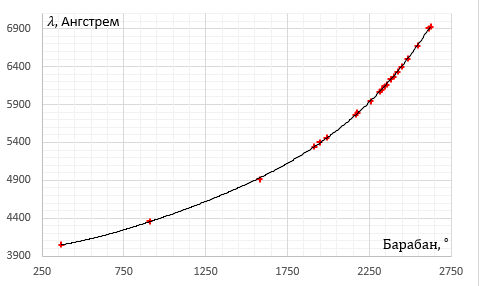
\includegraphics[width = 0.65\textwidth]{image/graph1.png}
        \caption{График калибровки барабана}
    \end{center}
\end{figure}

\subsection{Исследование спектров водорода и йода}

\begin{table}[!ht]
    \centering
    \begin{tabular}{|ccc|ccc|}
    \hline
    \multicolumn{3}{|c|}{\cellcolor[HTML]{DEE6EF}Водород}                                     & \multicolumn{3}{c|}{\cellcolor[HTML]{DEE6EF}Йод}                                         \\ \hline
    \multicolumn{1}{|c|}{Угол барабана, $^\circ$} & \multicolumn{1}{c|}{$\lambda$, \r{A}} & Полоса & \multicolumn{1}{c|}{Угол барабана, $^\circ$} & \multicolumn{1}{c|}{$\lambda$, \r{A}} & Полоса \\ \hline
    \multicolumn{1}{|c|}{2499}                   & \multicolumn{1}{c|}{6550}         & $H_\alpha$  & \multicolumn{1}{c|}{2338}                   & \multicolumn{1}{c|}{6140}         & $h\nu_{1,0}$    \\ \hline
    \multicolumn{1}{|c|}{1514}                   & \multicolumn{1}{c|}{4860}         & $H_\beta$   & \multicolumn{1}{c|}{2243}                   & \multicolumn{1}{c|}{5920}         & $h\nu_{1,5}$    \\ \hline
    \multicolumn{1}{|c|}{879}                    & \multicolumn{1}{c|}{4340}         & $H_\gamma$  & \multicolumn{1}{c|}{1840}                   & \multicolumn{1}{c|}{5245}         & $h\nu_{\text{гр}}$      \\ \hline
    \multicolumn{1}{|c|}{464}                    & \multicolumn{1}{c|}{4095}         & $H_\delta$  & \multicolumn{1}{c|}{1718}                   & \multicolumn{1}{c|}{5090}         & $h\nu_{\text{гр}}$      \\ \hline
    \end{tabular}
    \caption{Результаты измерений спектров водорода и йода}
\end{table}

\noindent В работе исследуется серия Бальмера: $n = 2$, $m = 3, 4, 5, 6$ для $H_{\alpha}, H_{\beta}, H_{\gamma}, H_{\delta}$ соответственно. Найдём значения~$R$ для различных линий водорода. Результаты представлены в таблице 3.

\begin{table}[!ht]
    \centering
    \begin{tabular}{|c|c|c|c|}
    \hline
    $\lambda$, \r{A} & Полоса       & $R$, \r{A}$^{-1}$ & $\sigma_R$, \r{A}$^{-1}$ \\ \hline
    $6550$                            & $H_{\alpha}$ & $1.099 \cdot 10^{-3}$              & $8.4 \cdot 10^{-7}$                       \\ \hline
    $4860$                            & $H_{\beta}$  & $1.097 \cdot 10^{-3}$              & $1.13 \cdot 10^{-6}$                      \\ \hline
    $4340$                            & $H_{\gamma}$ & $1.097 \cdot 10^{-3}$              & $1.26 \cdot 10^{-6}$                      \\ \hline
    $4095$                            & $H_{\delta}$ & $1.099 \cdot 10^{-3}$              & $1.34 \cdot 10^{-6}$                      \\ \hline
    \end{tabular}
    \caption{Результаты измерения постоянной Ридберга}
\end{table} 

\noindent Таким образом, получим
\begin{equation}
    R = (1.0980 \pm 0.0006) \cdot 10^{-3} \;\; \text{\r{A}}^{-1}.
\end{equation}

\noindent Используя калибровочный график (рис. 1), вычислим энергии для йода. Результаты представлены в таблице~4.
\begin{table}[!ht]
    \centering
    \begin{tabular}{|c|c|c|c|}
    \hline
    $\lambda$, \r{A} & Полоса             & $E$, эВ & $\sigma_E$, эВ      \\ \hline
    $6140$    & $h\nu_{1,0}$       & $2.020$  & $1.6 \cdot 10^{-3}$ \\ \hline
    $5920$    & $h\nu_{1,5}$        & $2.095$  & $1.8 \cdot 10^{-3}$ \\ \hline
    $5245$    & $h\nu_{\text{гр}}$ & $2.365$  & $2.3 \cdot 10^{-3}$ \\ \hline
    $5090$    & $h\nu_{\text{гр}}$ & $2.437$  & $2.4 \cdot 10^{-3}$ \\ \hline
    \end{tabular}
    \caption{Результаты измерения энергий кванта йода для различных спектральных линий}
\end{table}

\noindent Произведём рассчёты:
\begin{enumerate}
    \item $h\nu_2 = 0.015 \pm 0.002$ эВ --- энергия колебательного кванта возбужденного состояния молекулы йода.
    \item $h\nu_{\text{эл}} = h\nu_{1,5} - \frac{h\nu_1}{2} = 2.081 \pm 0.002$ эВ.
    \item $D_1 = h\nu_{\text{гр}} - E = 1.496 \pm 0.002$ эВ --- энергия диссоциации молекулы в основном состоянии ($E = 0.94$ эВ).
    \item $D_2 = h\nu_{\text{гр}} - h\nu_{\text{эл}} + 5.5 h\nu_2 = 0.4375$ эВ --- энергия диссоциации молекулы в возбужденном состоянии.
\end{enumerate}

\section{Вывод}
В работе были изучены спектры водорода и йода; экспериментально проверена справедливость формулы Бальмера и найдена постоянная Ридберга, которая хорошо приближает табличное значение ($R = 10 967 758,341$ м$^{-1}$); оценены энергии квантов возбужденного состояния молекулы, энергия диссоциации частиц и энергия электронного перехода.

\section{Приложение}

\begin{figure}[!ht]
    \begin{center}
        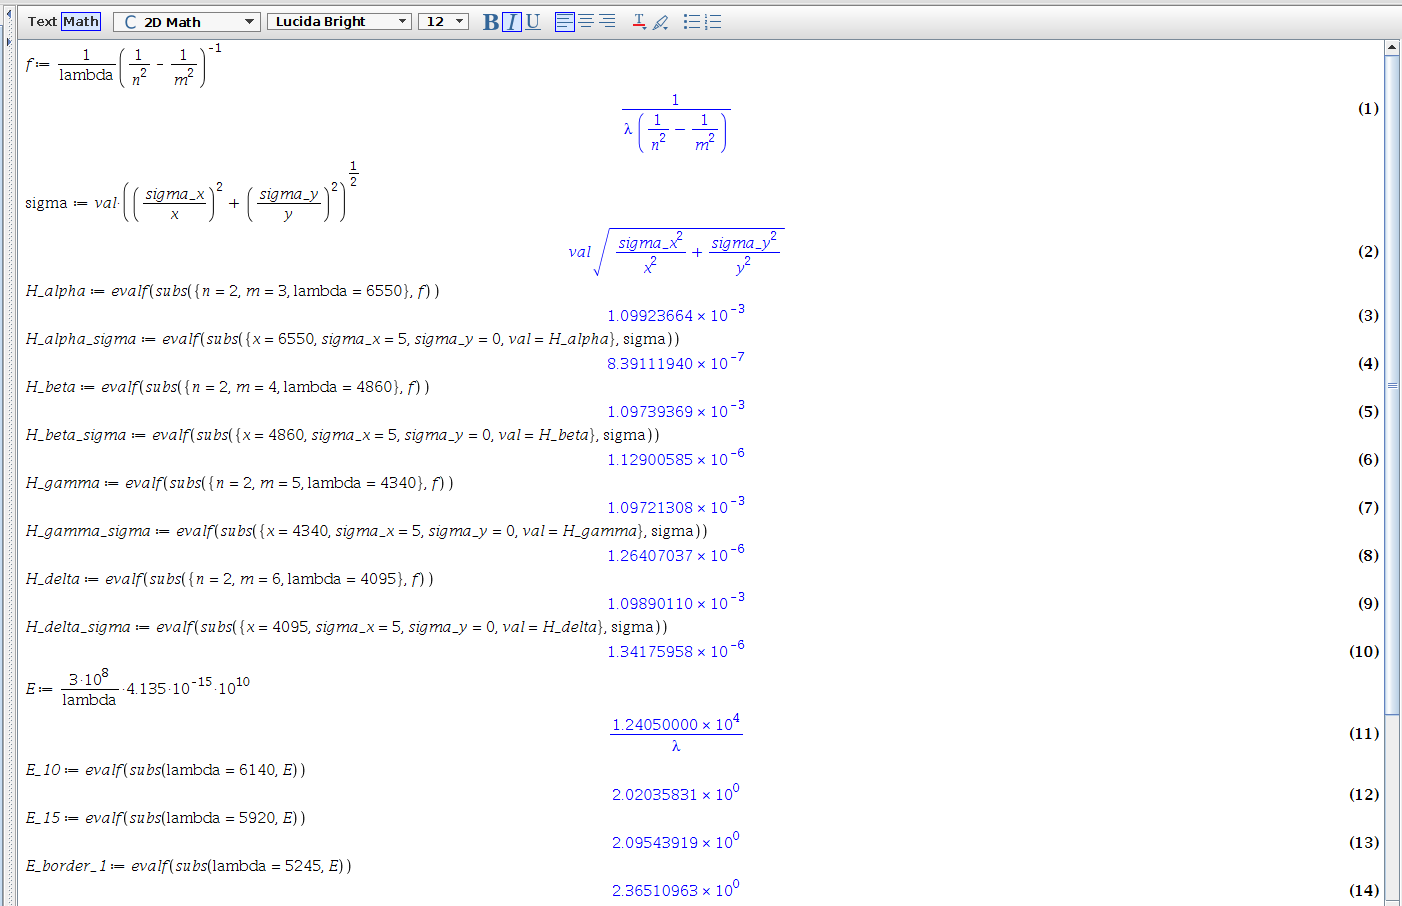
\includegraphics[width = 0.78\textwidth]{image/maple1.png}
        \caption{Подсчёт величин и их погрешностей}
    \end{center}
\end{figure}

\begin{figure}[!ht]
    \begin{center}
        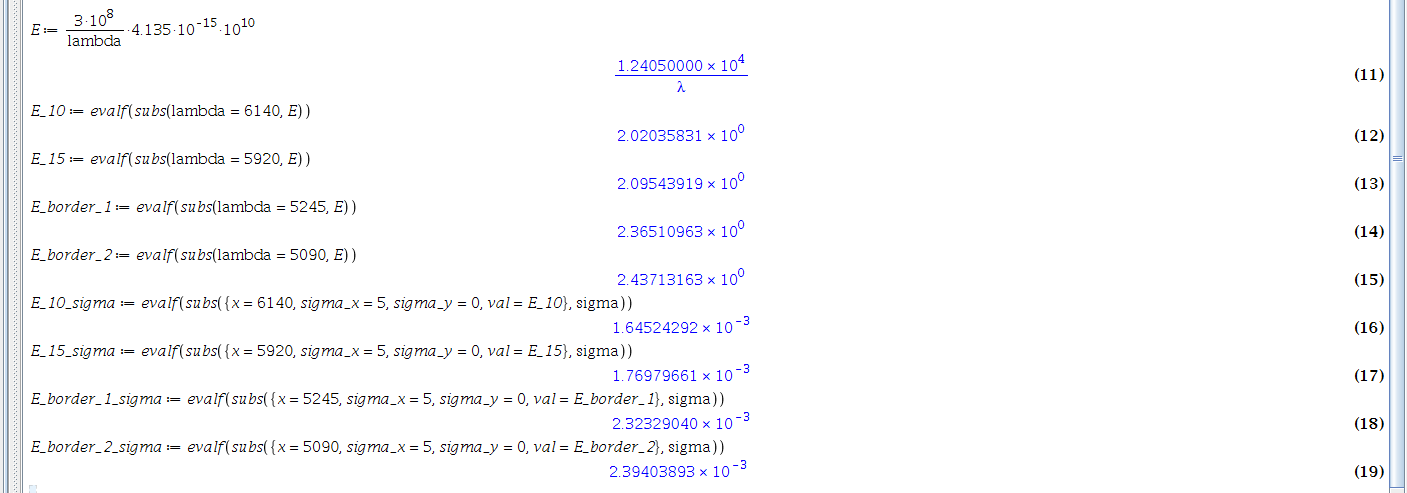
\includegraphics[width = 0.78\textwidth]{image/maple2.png}
        \caption{Подсчёт величин и их погрешностей}
    \end{center}
\end{figure}

\end{document}
